%%%%%%%%%%%%%%%%%%%%%%%%%%%%%%%%%%%%%%%%%
% Beamer Presentation
% LaTeX Template
% Version 1.0 (10/11/12)
%
% This template has been downloaded from:
%----------------------------------------------------------------------------------------

\documentclass[aspectratio=169]{beamer}
%%\documentclass{beamer}
\usetheme{Madrid}
\usepackage{todonotes}
\usepackage{graphicx}
\usepackage{xcolor}
\usepackage{subfig}
%%\usepackage[noend]{algpseudocode}


\usepackage{algorithm}
\usepackage{algorithmic}

\usepackage{blkarray}
\usepackage{amsmath}
\usepackage{xspace}
\usepackage{float}




\usepackage{tikz}
\usetikzlibrary{matrix, decorations, patterns, positioning, shapes, calc, intersections, arrows, fit, hobby}
%%\usepackage{enumitem}

\mode<presentation> {

% The Beamer class comes with a number of default slide themes
% which change the colors and layouts of slides. Below this is a list
% of all the themes, uncomment each in turn to see what they look like.

%\usetheme{default}
%\usetheme{AnnArbor}
%\usetheme{Antibes}
%\usetheme{Bergen}
%\usetheme{Berkeley}
%\usetheme{Berlin}
%\usetheme{Boadilla}
%\usetheme{CambridgeUS}
%\usetheme{Copenhagen}
%\usetheme{Darmstadt}
%\usetheme{Dresden}
%\usetheme{Frankfurt}
%\usetheme{Goettingen}
%\usetheme{Hannover}
%\usetheme{Ilmenau}
%\usetheme{JuanLesPins}
%\usetheme{Luebeck}
\usetheme{Madrid}
%\usetheme{Malmoe}
%\usetheme{Marburg}
%\usetheme{Montpellier}
%\usetheme{PaloAlto}
%\usetheme{Pittsburgh}
%\usetheme{Rochester}
%\usetheme{Singapore}
%\usetheme{Szeged}
%\usetheme{Warsaw}

% As well as themes, the Beamer class has a number of color themes
% for any slide theme. Uncomment each of these in turn to see how it
% changes the colors of your current slide theme.

%\usecolortheme{albatross}
%\usecolortheme{beaver}
%\usecolortheme{beetle}
%\usecolortheme{crane}
%\usecolortheme{dolphin}
%\usecolortheme{dove}
%\usecolortheme{fly}
%\usecolortheme{lily}
%\usecolortheme{orchid}
%\usecolortheme{rose}
%\usecolortheme{seagull}
%\usecolortheme{seahorse}
%\usecolortheme{whale}
%\usecolortheme{wolverine}

%\setbeamertemplate{footline} % To remove the footer line in all slides uncomment this line
%\setbeamertemplate{footline}[page number] % To replace the footer line in all slides with a simple slide count uncomment this line

%\setbeamertemplate{navigation symbols}{} % To remove the navigation symbols from the bottom of all slides uncomment this line
}


\usepackage{booktabs} % Allows the use of \toprule, \midrule and \bottomrule in tables


\newcommand{\tensor}[1]{\T{#1}}
\newcommand{\lowerbound}{{\sc C_{LB}}\xspace}
\newcommand{\maxp}{{\sc MaxP}\xspace}
\newcommand{\lowerboundmatrix}{{\sc LB(MatrixComm)}\xspace}
\newcommand{\lowerboundtensor}{{\sc LB(TensorComm)}\xspace}
\newcommand{\odata}{{\sc O_d}\xspace}
\newcommand{\init}[1]{\hat{#1}}
\newcommand{\tmp}[1]{q_{prev}}
\newcommand{\lbbasedpartition}{{\it Algo1($C_{LB}$ based config)}\xspace}
\newcommand{\bestconfigAAO}{{\it Algo1(best config)}\xspace}
\newcommand{\bestconfigSeq}{{\it Seq-Appr(best config)}\xspace}

%% Colors from https://latexcolor.com/
\definecolor{pastelviolet}{rgb}{0.8, 0.6, 0.79}
\definecolor{babyblueeyes}{rgb}{0.63, 0.79, 0.95}
\definecolor{pastelyellow}{rgb}{0.99, 0.99, 0.59}
\definecolor{pastelgreen}{rgb}{0.47, 0.87, 0.47}
\definecolor{pastelred}{rgb}{1.0, 0.41, 0.38}
\colorlet{patternblue}{blue!60}


%%For tensor notations
\input{./tensor_header}
\newcommand{\X}{\T{X}}
\newcommand{\Y}{\T{Y}}
\newcommand{\starontop}[1]{{#1}^*}


\graphicspath{{./diagrams/}{./Figs/}{./plots/}}

%%\newenvironment{beameritemize}
%%{ \begin{itemize}
%%		\setlength{\itemsep}{1.5ex}
%%		\setlength{\parskip}{0pt}
%%		\setlength{\parsep}{0pt}   
%%		\addtolength{\itemindent}{-2em}  }
%%{ \end{itemize} }


%----------------------------------------------------------------------------------------
%	TITLE PAGE
%----------------------------------------------------------------------------------------

\title[Multi-TTM Computation]{Communication Optimal Algorithms for Multiple
	Tensor-Times-Matrix Computation} % The short title appears at the bottom of every slide, the full title is only on the title page

%%\author{John Smith} % Your name
%%\institute[UCLA] % Your institution as it will appear on the bottom of every slide, may be shorthand to save space
%%{
%%University of California \\ % Your institution for the title page
%%\medskip
%%\textit{john@smith.com} % Your email address
%%}
\author[Suraj {\sc Kumar}]{Hussam {\sc Al Daas}\inst{1}, Grey {\sc Ballard}\inst{2}, Laura {\sc Grigori}\inst{3}, \underline{Suraj {\sc Kumar}}\inst{3}, and Kathryn {\sc Rouse}\inst{4}}

%%\underline{Suraj {\sc Kumar}}\inst{1}, Lionel {\sc Eyraud-Dubois}\inst{2}, and\\ Sriram {\sc Krishnamoorthy}\inst{1}}
\institute[Inria Paris]{\inst{1} Rutherford Appleton Laboratory, UK \and %
	\inst{2} Wake Forest University, USA \and
    \inst{3} Inria Paris, France \and
    \inst{4} Inmar Intelligence, USA}
\date[ROMA Working Group]{ROMA Working Group\\\today} % Date, can be changed to a custom date

\begin{document}

\begin{frame}
\titlepage % Print the title page as the first slide
\end{frame}

\begin{frame}{My Past Experience}

{\scriptsize
\vspace*{-0.15cm}\begin{columns}
	\begin{column}{0.31\linewidth}
		\begin{block}{\footnotesize Parallelization in Polyhedral Model}
			\begin{columns}
				\begin{column}{0.56\linewidth}
%%					{\scriptsize
%%					$\bullet$ Linked-list operations\\
%%					$\bullet$ Improved spatial locality}
					\begin{itemize}{\scriptsize
						\item Linked-list operations
						\item Improved spatial locality
%%				  	    \item Analyze dependencies among operations
						\item Parallelization using OpenMP
					}\end{itemize}
				\end{column}
				\begin{column}{0.425\linewidth}
					\begin{center}
						\includegraphics[scale=0.725]{PolyhedralFramework.png}
					\end{center}
				\end{column}
			\end{columns}
		\end{block}
	\end{column}
	\begin{column}{0.3\linewidth}
		\begin{block}{\footnotesize Seismic Imaging on GPUs}{\tiny
			\vspace*{-0.56cm}\begin{align*}
			H_1 =& \sin^2\theta \cos^2 \phi \frac{\partial^2}{\partial x^2} + \sin^2\theta \sin^2\phi \frac{\partial^2}{\partial y^2}\\ &+ \cos^2 \theta \frac{\partial^2}{\partial z^2}
		    + \sin^2 \theta \sin 2\phi \frac{\partial^2}{\partial x \partial y}\\ & + \sin 2\theta\sin\phi \frac{\partial^2}{\partial y\partial z} + \sin 2\theta \cos \phi \frac{\partial^2}{\partial x \partial z}\\
			H_2 = & \frac{\partial^2}{\partial x^2} + \frac{\partial^2}{\partial y^2} + \frac{\partial^2}{\partial z^2} - H_1
%%			\frac{\partial^2 p}{\partial t^2} = v_{px}^2 H_2p + \alpha v_{pz}^2 H_1q + v_{sz}^2 H_1(p-\alpha q)\\
%%			\frac{\partial ^2 q}{\partial t^2} = \frac{v_{pn}^2}{\alpha}H_2p + \alpha v_{pz}^2 H_1q - v_{sz}^2 H_2(\frac{p}{\alpha} - q)
			\end{align*}\vspace*{-0.5cm}
%%			∂2p∂2t=v2pxH2p+αv2pzH1q+v2szH1(p−αq)∂2q∂2t=v2pnαH2p+αv2pzH1q−v2szH2(1αp−q)
%%			\begin{center}
%%				\includegraphics[scale=0.425]{PolyhedralFramework.png}
%%			\end{center}
	}\end{block}
	\end{column}
	\begin{column}{0.345\linewidth}
		\begin{block}{\footnotesize Schedulers for Blue Gene Supercomputers}
			\begin{columns}
				\begin{column}{0.5\linewidth}
					\begin{itemize}{\scriptsize
						\item GASNET API
						\item Unbalanced Tree Search benchmark
						\item Comparison to Charm++
					}\end{itemize}
				\end{column}
				\begin{column}{0.45\linewidth}
					\begin{center}
						\includegraphics[scale=0.25]{IBM_Blue_Gene_P_supercomputer.jpg}
					\end{center}
				\end{column}
			\end{columns}
		\end{block}
	\end{column}
\end{columns}
\vfill
\begin{columns}
	\begin{column}{0.475\linewidth}
		\begin{block}{\footnotesize Scheduling on Heterogeneous Platforms}
			\begin{center}
%%				\includegraphics[scale=0.2]{taskGraph.eps}
				\includegraphics[scale=0.095]{Cholesky-4.pdf}$\qquad$
				\includegraphics[scale=0.145]{HeterogenousPlatform.png}
			\end{center}
		\end{block}
	\end{column}
	\begin{column}{0.475\linewidth}
		\begin{block}{\footnotesize Molecular Simulations on Supercomputers}
			\begin{columns}
				\begin{column}{0.35\linewidth}
					\begin{itemize}{\scriptsize
						\item NWChemEx Project
						\item TAMM library
						\item Hartree Fock and CCSD applications
					}\end{itemize}
				\end{column}
				\begin{column}{0.6\linewidth}
					\vspace*{-0.4cm}\begin{center}
						\includegraphics[scale=0.07]{SummitNode.jpg}
					\end{center}\vspace*{-0.375cm}
				\end{column}
			\end{columns}
		\end{block}
	\end{column}
\end{columns}
}
\end{frame}

\begin{frame}
\titlepage % Print the title page as the first slide
\end{frame}



%%\begin{frame}{Introduction}
%%\begin{itemize}
%%	\item Accelerators are becoming standard in HPC community
%%	\begin{itemize}
%%		\item Provide massive computational power at a limited cost 
%%		\item 144 systems in TOP 500 list use accelerators
%%	\end{itemize}
%%	\item  Exploiting the full potential of hybrid platforms is challenging
%%	\begin{itemize}
%%		\item Difficult to precisely model computation and data transfer times
%%		\item Scheduling 
%%%%		on these platforms 
%%			  is a well known hard optimization problem
%%	\end{itemize}
%%%%	\item Asynchronous task based runtime systems show promising performance on hybrid platforms.
%%	\item Task based runtime systems are getting popular to make good utilization of resources
%%			\begin{columns}
%%		\null \hfill
%%		\begin{column}{0.35\linewidth}
%%			\begin{center}
%%%%				\includegraphics[scale=0.2]{taskGraph.eps}
%%				\includegraphics[scale=0.12]{Cholesky-4.pdf}
%%			\end{center}
%%		\end{column}
%%		\begin{column}{0.65\linewidth}
%%			\begin{itemize}
%%				\item Applications can be expressed as task graphs
%%				\item Vertices represent tasks
%%				\item Edges represent dependencies among tasks
%%				\item Runtime manages scheduling of computations and communications
%%			\end{itemize}
%%		\end{column}
%%		\end{columns}
%%	 
%%\end{itemize}
%%\end{frame}

\begin{frame}{Higher-order SVD (HOSVD) to compute Tucker decomposition}
\begin{center}
	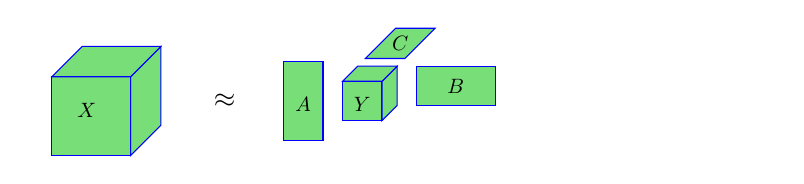
\begin{tikzpicture}[scale=0.25, every node/.style={transform shape}]
	\pgfmathsetmacro{\cubex}{4}
	\pgfmathsetmacro{\cubey}{4}
	\pgfmathsetmacro{\cubez}{4}
	\draw[blue,fill=pastelgreen] (-12,1,\cubez-2) -- ++(-\cubex,0,0) -- ++(0,-\cubey,0) -- ++(\cubex,0,0) -- cycle;
	\node [scale=3] at (-15,-1.5, 0) {$\X$};
	\draw[blue,fill=pastelgreen] (-12,1,\cubez-2) -- ++(0,0,-\cubez) -- ++(0,-\cubey,0) -- ++(0,0,\cubez) -- cycle;
	\draw[blue,fill=pastelgreen] (-12,1,\cubez-2) -- ++(-\cubex,0,0) -- ++(0,0,-\cubez) -- ++(\cubex,0,0) -- cycle;
	\node[draw=none, text=black, scale=4] at (-8,-1,0) {$\approx$};
	
	\pgfmathsetmacro{\cubex}{2}
	\pgfmathsetmacro{\cubey}{2}
	\pgfmathsetmacro{\cubez}{2}
	\draw[blue,fill=pastelgreen] (0,0,0) -- ++(-\cubex,0,0) -- ++(0,-\cubey,0) -- ++(\cubex,0,0) -- cycle;
	\draw[blue,fill=pastelgreen] (0,0,0) -- ++(0,0,-\cubez) -- ++(0,-\cubey,0) -- ++(0,0,\cubez) -- cycle;
	\draw[blue,fill=pastelgreen] (0,0,0) -- ++(-\cubex,0,0) -- ++(0,0,-\cubez) -- ++(\cubex,0,0) -- cycle;
	
	\node [scale=3] at (-1, -1.2, 0) {$\Y$};
	\draw[blue,fill=pastelgreen] (-\cubex-1,1,0) -- ++(-\cubex,0,0) -- ++(0,-\cubey-2,0) -- ++(\cubex,0,0) -- cycle;
	
	\node [scale=3] at (-4, -1.2, 0) {$A$};
	
	\draw[blue,fill=pastelgreen] (\cubex+2+1,0,-\cubey) -- ++(-\cubex-2,0,0) -- ++(0,-\cubey,0) -- ++(\cubex+2,0,0) -- cycle;
	\node [scale=3] at (3.75, -0.25, 0) {$B$};
	
	\draw[blue,fill=pastelgreen] (0,0,-\cubez-1) -- ++(-\cubex,0,0) -- ++(0,0,-\cubez-2) -- ++(\cubex,0,0) -- cycle;
	\node [scale=3] at (-1, 0, -5) {$C$};
	
	\path (-18,0) -- (20,0);
	\end{tikzpicture}

{\footnotesize
\begin{algorithm}[H]{\footnotesize
	\caption{HOSVD Algorithm($\X$, $R_1$, $R_2$, $R_3$)}
	\begin{algorithmic}[1]
		\STATE $A \leftarrow$ $R_1$ left singular vectors of $\X_{(1)}$
		\STATE $B \leftarrow$ $R_2$ left singular vectors of $\X_{(2)}$
		\STATE $C \leftarrow$ $R_3$ left singular vectors of $\X_{(3)}$
		\STATE $\Y = \X \times_1 A^\Tra \times_2 B^\Tra \times_3 C^\Tra$
		\STATE Return $\Y$, $A$, $B$, $C$
	\end{algorithmic}
}\end{algorithm}

\vspace*{-0.45cm}
\begin{itemize}
	\item $\X$, $\Y$: 3-dimensional input and output tensors (or arrays) \& $A$, $B$, $C$: matrices
	\item $\X_{(i)}$: matricization of $\X$ ($i$th dimension represents rows and remaining dimensions represent columns)
	\item Multiple Tensor-Times-Matrix (Multi-TTM) computation: $\Y = \X \times_1 A^\Tra \times_2 B^\Tra \times_3 C^\Tra$
	\begin{itemize}
		\item To obtain full tensor, $\X = \Y \times_1 A \times_2 B \times_3 C$
	\end{itemize}
\end{itemize}
}
%%	\begin{algorithm}[H]
%%		\caption{\label{alg:3dmultittm}3-dimensional Parallel Atomic Multi-TTM}
%%		\begin{algorithmic}[1]
%%			\REQUIRE $\T{X}$, $\Mn{A}{1}$, $\Mn{A}{2}$, $\Mn{A}{3}$, $p_1 \times p_2 \times p_3 \times q_1 \times q_2 \times q_3$ logical processor grid
%%			\ENSURE $\T{Y}$ such that $\Y = \X \times_1 {\Mn{A}{1}}^\Tra \times_2 {\Mn{A}{2}}^\Tra \times_3 {\Mn{A}{3}}^\Tra$
%%			\STATE $(p_1^\prime, p_2^\prime, p_3^\prime, q_1^\prime, q_2^\prime, q_3^\prime)$ is my processor id
%%			\STATE //All-gather input tensor $\T{X}$
%%			\STATE $\T{X}_{p_1^\prime p_2^\prime p_3^\prime}$ = All-Gather($\T{X}$, $(p_1^\prime, p_2^\prime, p_3^\prime, *, *, *)$)\label{alg:3dmultittm:line:allGatherInputTensor}
%%			\STATE //All-gather input matrices
%%			\STATE $\Mn{A}{1}_{p_1^\prime q_1^\prime}$ = All-Gather($\Mn{A}{1}$, $(p_1^\prime, *, *, q_1^\prime, *, *)$)\label{alg:3dmultittm:line:allGatherMatrix1}
%%			\STATE $\Mn{A}{2}_{p_2^\prime q_2^\prime}$ = All-Gather($\Mn{A}{2}$, $(*, p_2^\prime, *, *, q_2^\prime, *)$)\label{alg:3dmultittm:line:allGatherMatrix2}
%%			\STATE $\Mn{A}{3}_{p_3^\prime q_3^\prime}$ = All-Gather($\Mn{A}{3}$, $(*, *, p_3^\prime, *, *, q_3^\prime)$)\label{alg:3dmultittm:line:allGatherMatrix3}
%%			\STATE //Perform local Multi-TTM computation in a temporary tensor $\T{T}$
%%			\STATE $\T{T}$ = Local-Multi-TTM($\T{X}_{p_1^\prime p_2^\prime p_3^\prime}$, $\Mn{A}{1}_{p_1^\prime q_1^\prime}$, $\Mn{A}{2}_{p_2^\prime q_2^\prime}$, $\Mn{A}{3}_{p_3^\prime q_3^\prime}$)\label{alg:3dmultittm:line:localcomputation}
%%			\STATE //Reduce-scatter the output tensor in $\T{Y}_{q_1^\prime q_2^\prime q_3^\prime}$
%%			\STATE Reduce-Scatter($\T{Y}_{q_1^\prime q_2^\prime q_3^\prime}$, $\T{T}$, $(*, *, *, q_1^\prime, q_2^\prime, q_3^\prime)$)\label{alg:3dmultittm:line:reduceScatterOutputTensor}
%%		\end{algorithmic}
%%	\end{algorithm}
\end{center}

%% $\X = \Y \times_1 {\Mn{A}{1}} \cdots \times_d {\Mn{A}{d}}$ to obtain the full tensor or as $\Y = \X \times_1 {\Mn{A}{1}}^\Tra \cdots \times_d {\Mn{A}{d}}^\Tra$
\end{frame}
\begin{frame}
\frametitle{Outline (Lower Bounds and Communication Optimal Algorithms)} % Table of contents slide, comment this block out to remove it
\tableofcontents % Throughout your presentation, if you choose to use \section{} and \subsection{} commands, these will automatically be printed on this slide as an overview of your presentation

\begin{block}{Assumptions}
	\begin{itemize}
		\item $P$ number of processors
		\item Each processor performs (asymptotically) equal amount of operations
		\item No redundant operations
		\item One copy of data is in the system
		\begin{itemize}
			\item $1/P$th amount of inputs (before the computation) and output (after the computation) on each processor  
		\end{itemize}
		\item Each processor has enough memory
	\end{itemize}
\end{block}
\end{frame}
\section{For Matrix Matrix Multiplications}

\begin{frame}{Outline (Lower Bounds and Communication Optimal Algorithms)}
\tableofcontents[currentsection]
\end{frame}
\begin{frame}{Existing Lower Bounds for Matrix Matrix Multiplications}
\begin{itemize}
	\item $C=AB$, where $A \in \mathbb{R}^{n_1\times n_2}, B \in \mathbb{R}^{n_2\times n_3}$, and $C \in \mathbb{R}^{n_1\times n_3}$
	\item Let $d_1=\min(n_1,n_2,n_3) \le d_2=median(n_1,n_2,n_3) \le d_3 = \max(n_1,n_2,n_3)$
\end{itemize}

\begin{minipage}{0.7\linewidth}
	\begin{block}{\small Existing Communication Lower Bounds (CARMA [IPDPS 2013])}
	\begin{center}
	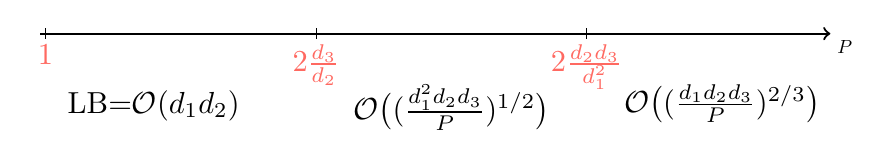
\begin{tikzpicture}[scale=0.6875, every node/.style={transform shape}]
	%%\draw (-2,0) -- node[below] {a} ++(2,0) -- node[above] {b} ++(2,0);
	%%\draw (-0.1,0) -- ++(5,0) -- ++(5,0);
	\draw [->, thick] (-0.1,0) -- (14.5,0) node [below right] {$P$};
	\draw (0, 0.1) -- node [below, pastelred, scale=1.6]{$1$}(0,-0.1);
	\draw (5, 0.1) -- node [below, pastelred, scale=1.6]{$2\frac{d_3}{d_2}$}(5,-0.1);
	\draw (10, 0.1) -- node [below, pastelred, scale=1.6] {$2\frac{d_2d_3}{d_1^2}$}(10,-0.1);
	
	\node[align=left,below,scale=1.6] at (2, -0.85) {LB=$\mathcal{O}(d_1d_2)$};
	\node[align=left,below,scale=1.6] at (7.5, -0.75) {$\mathcal{O}\big((\frac{d_1^2d_2d_3}{P})^{1/2}\big)$};
	\node[align=center,below,scale=1.6] at (12.5, -0.75) {$\mathcal{O}\big((\frac{d_1d_2d_3}{P})^{2/3}\big)$};	
	\end{tikzpicture}
	\end{center} 
	\end{block}
	\only<2>{\begin{alertblock}{\small Our Communication Lower Bounds}
		\begin{center}
			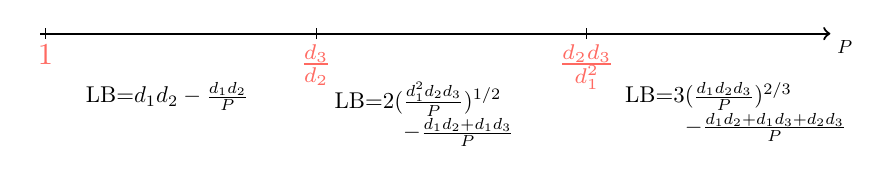
\begin{tikzpicture}[scale=0.6875, every node/.style={transform shape}]
			%%\draw (-2,0) -- node[below] {a} ++(2,0) -- node[above] {b} ++(2,0);
			%%\draw (-0.1,0) -- ++(5,0) -- ++(5,0);
			\draw [->, thick] (-0.1,0) -- (14.5,0) node [below right] {$P$};
			\draw (0, 0.1) -- node [below, pastelred, scale=1.6]{$1$}(0,-0.1);
			\draw (5, 0.1) -- node [below, pastelred, scale=1.6]{$\frac{d_3}{d_2}$}(5,-0.1);
			\draw (10, 0.1) -- node [below, pastelred, scale=1.6] {$\frac{d_2d_3}{d_1^2}$}(10,-0.1);
			
			\node[align=left,below,scale=1.2] at (2.25, -0.75) {LB=$d_1d_2 -\frac{d_1d_2}{P}$};
			\node[align=left,below,scale=1.2] at (7, -0.75) {LB=$2(\frac{d_1^2d_2d_3}{P})^{1/2}$\\
				$\qquad\quad-\frac{d_1d_2+d_1d_3}{P}$};
			\node[align=center,below,scale=1.2] at (12.25, -0.75) {LB=$3(\frac{d_1d_2d_3}{P})^{2/3}$\\ $\qquad\qquad\quad -\frac{d_1d_2+d_1d_3+d_2d_3}{P}$};	
			\end{tikzpicture}
		\end{center} 
	\end{alertblock}}
\end{minipage}$\quad$
\begin{minipage}{0.25\linewidth}
	\begin{exampleblock}{\small Arrangements of $8$ processors}
		\begin{center}
			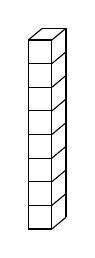
\begin{tikzpicture}[scale=0.3, every node/.style={transform shape}]	
			\foreach \x in {0, 1, 2, 3, 4, 5, 6, 7, 8}
			\draw (-1, \x) -- (0, \x);
			
			\foreach \x in {0, 1, 2, 3, 4, 5, 6, 7, 8}
			\draw (0, \x)--(0.6, 0.5+\x);
			
			\draw (0,0) -- (0,8);
			\draw(-1,0)--(-1,8);
			\draw (0.6,0.5) -- (0.6,8.5);
			\draw (-1,8) -- (-1+0.6,8.5);
			
			\draw (-1+0.6,8.5) -- (0.6,8.5);
			
			\end{tikzpicture}$\quad$
			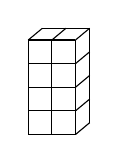
\begin{tikzpicture}[scale=0.3, every node/.style={transform shape}]
			
			\foreach \x in {0, 1, 2, 3, 4}
			\draw (-2, \x) -- (0, \x);
			
			\foreach \x in {0, 1, 2, 3, 4}
			\draw (0, \x)--(0.6, 0.5+\x);
			
			\draw (0,0) -- (0,4);
			\draw (-1,0) -- (-1,4);
			\draw(-2,0)--(-2,4);
			
			\draw (0.6,0.5) -- (0.6,4.5);
			
			\draw (-2,4) -- (-2+0.6, 4+0.5);
			\draw (-2+0.6, 4+0.5) -- (0.6, 4.5);
			
			\draw (-1,4) -- (-1+0.6, 4+0.5);
			
			%%\draw (-1,8) -- (0,8.5);
			%%\draw (0,8.5) -- (1,8.5);
			
			\end{tikzpicture}$\quad$
			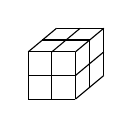
\begin{tikzpicture}[scale=0.3, every node/.style={transform shape}]
			
			\def\xref{0.6}
			\def\yref{0.5}
			
			\foreach \x in {0, 1, 2}
			\draw (-2, \x) -- (0, \x);
			
			\foreach \x in {0, 1, 2}
			\draw (0, \x)--(2*\xref, 2*\yref+\x);
			
			\draw (0,0) -- (0,2);
			\draw (-1,0) -- (-1,2);
			\draw (-2,0)--(-2,2);
			\draw (\xref,\yref) -- (\xref, 2+\yref);
			\draw (2*\xref,2*\yref) -- (2*\xref, 2+ 2*\yref);
			
			\draw (-2,2) -- (-2+2*\xref, 2+2*\yref);
			\draw (-1,2) -- (-1+2*\xref, 2+2*\yref);
			
			\draw (-2+2*\xref, 2+2*\yref) -- (2*\xref, 2+2*\yref);
			\draw (-2+\xref, 2+\yref) -- (\xref, 2+\yref);
			\end{tikzpicture}
		\end{center}
	\end{exampleblock}
\end{minipage}
\end{frame}
\begin{frame}{Loomis-Whitney \&  H\"{o}lder-Brascamp-Lieb inequalities}
\vspace*{-0.25cm}\begin{block}{\small Size of $d-1$ dimensional projections (Loomis-Whitney inequalitiy)}
	\begin{minipage}{0.375\linewidth}
		\vspace*{-0.35cm}\begin{block}{}
		\begin{columns}
			\begin{column}{0.6\linewidth}
				\vspace*{-0.45cm}\begin{itemize}{\footnotesize
						\item $2$-dimensional object $A$ and its $1$-dimensional projections $\phi_x$, $\phi_y$
						\item $\phi_x \phi_y \ge Area(A)$
				}\end{itemize}		
			\end{column}
			\begin{column}{0.35\linewidth}
					\begin{center}
					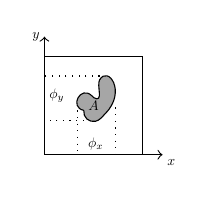
\begin{tikzpicture}[scale=0.25, every node/.style={transform shape}]
					\draw (0,0) -- ++(5,0) -- ++(0, 5) -- ++(-5,0) -- cycle;
					\draw [<->] (0,6) -- (0,0) -- (6,0);
					\node [below right, scale=2] at (6,0) {$x$};
					\node [left, scale=2] at (0,6) {$y$};
					
					\draw [fill=gray!70] (2,2.25) to [curve through={(2.4,3) .. (2.5,2.9) .. (2.8,3.8) .. (3.1,2.1) .. (2.6,1.7)}] (2,2.25);
					
					\node [scale=2] at (2.5,2.5) {$A$};
					\draw [dotted] (1.7,2.25) -- (1.7,0);
					\draw [dotted] (3.6,2.4) -- (3.6,0);
					
					\node[above, scale=2] at (2.6,0) {$\phi_x$};
					
					\draw [dotted] (2,1.75) -- (0,1.75);
					\draw [dotted] (2.8,4) -- (0,4);
					
					\node[right, scale=2] at (0,3) {$\phi_y$};
					\end{tikzpicture}
				\end{center}
			\end{column}
		\end{columns}

%%		\vspace*{-0.75cm}
		\end{block}
	\end{minipage}$\quad$
	\begin{minipage}{0.56\linewidth}
	\vspace*{-0.35cm}\begin{block}{}
		\begin{columns}
			\begin{column}{0.6\linewidth}
				\vspace*{-0.4cm}\begin{itemize}{\footnotesize
						\item $3$-dimensional object $A$ and its $2$-dimensional projections: $\phi_{xy}$, $\phi_{yz}$, $\phi_{xz}$
						\item $(\phi_{xy}\phi_{yz}\phi_{xz})^\frac{1}{3-1} \ge Volume(A)$
				}\end{itemize}
			\end{column}
			\begin{column}{0.35\linewidth}
					\begin{center}
					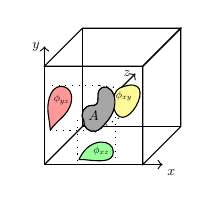
\begin{tikzpicture}[scale=0.25, every node/.style={transform shape}]
					\draw (0,0) -- ++(5,0) -- ++(0, 5) -- ++(-5,0) -- cycle;
					\draw (0,5,0) -- ++(0,0, -5) -- ++(5,0,0) -- ++(0,0,5) -- cycle;
					\draw (5,0,0) -- ++(0,0,-5) -- ++(0,5,0) -- ++(0,0,5) -- cycle;
					\draw (0,0,-5) -- ++(5,0,0) -- ++(0,5,0) -- ++(-5,0,0) -- cycle;
					\draw [<->] (0,6) -- (0,0) -- (6,0);
					\draw [->] (0,0,0) -- (0,0,-12);
					\node [left, scale=2, rotate=0] at (0,0,-12) {$z$};
					\node [below right, scale=2] at (6,0) {$x$};
					\node [left, scale=2] at (0,6) {$y$};
					
					\draw [fill=gray!70] (2,2.25) to [curve through={(2.4,3) .. (2.5,3) .. (2.8,3.8) .. (3.1,2.1) .. (2.6,1.7)}] (2,2.25);
					
					\node [scale=2] at (2.5,2.5) {$A$};
					\draw [dotted] (1.7,2.25) -- (1.7,0.2);
					\draw [dotted] (3.6,2.4) -- (3.6,0.3);
					
					\draw [fill=green!40] (1.75,0.25) to [curve through={(1.8, 0.35) .. (3.5, 0.65) .. (2,0.25)}] (1.75,0.25);
					\node[above, scale=1.5] at (2.6,0,-0.75) {$\phi_{xz}$};
					
					\draw [dotted] (2,1.75) -- (0.3,1.75);
					\draw [dotted] (2.8,4) -- (0.385,4);
					
					\draw [fill=red!40] (0.3, 1.75) to [curve through={(0.5,2) .. (1, 2.5) .. (1,3.95) .. (0.2, 2.5)}] (0.3,1.75);
					\node[right, scale=1.5] at (0,3, -0.75) {$\phi_{yz}$};
					
					\draw [fill=yellow!40] (3.85,3.9) to [curve through={(3.7,3.8) .. (3.5,3.4) .. (3.45,3.2)}] (3.85, 3.9);
					\node [scale=1.5] at (3.65,3.1,-1) {$\phi_{xy}$};
					\draw [dotted] (2.8,4) -- (3.8,3.9);
					\draw [dotted] (2.56,1.65) -- (4,2.5);
					
					\draw [fill=gray!70] (2,2.25) to [curve through={(2.4,3) .. (2.5,3) .. (2.8,3.8) .. (3.1,2.1) .. (2.6,1.7)}] (2,2.25);
					
					\node [scale=2] at (2.5,2.5) {$A$};
					\end{tikzpicture}
				\end{center}
			\end{column}
		\end{columns}
%%		\vspace*{-0.85cm}
	\end{block}
\end{minipage}\vspace*{-0.1cm}
\end{block}
\vspace*{-0.325cm}\begin{block}{\small H\"{o}lder-Brascamp-Lieb (HBL) inequality -- Generalization of Loomis-Whitney inequality}
	\begin{columns}
		\begin{column}{0.35\linewidth}{\small
			\vspace*{-0.5cm}\begin{center}
				$\M{\Delta} = \begin{blockarray}{cccc}
				& A & B & C  \\
				\begin{block}{c(ccc)}
				i & 1 & 0 & 1\\
				j & 0 & 1 & 1\\
				k & 1 & 1 & 0\\
				\end{block}
				\end{blockarray}$
			\end{center}
		}\end{column}
		\begin{column}{0.6\linewidth}
			\vspace*{-0.35cm}\begin{align*}
			&\text{for $i = 1{:}n_1$, for $k = 1{:}n_2$, for $j = 1{:}n_3$}\\
			&\quad \quad C[i][j] += A[i][k]*B[k][j]
			\end{align*}
		\end{column}
	\end{columns}
	\vspace*{-0.6cm}\begin{itemize}{\small
			\item Find $\V{x}=\begin{bmatrix} x_1 & x_2 & x_3 \end{bmatrix}^\Tra$ such that $\M{\Delta}.\V{x} \ge \V{1}$, $\V{1}$ is vector of all ones
			\item $\phi_A, \phi_B, \phi_C$: projections of computations on arrays $A$, $B$, $C$
			\item HBL inequality:  $\phi_A^{x_1} \phi_B^{x_2} \phi_C^{x_3} \ge \text{Amount of computations}$
			\item To make inequality tight select $\V{x}$ such that $\V{1}^\Tra \V{x}$ is minimum $=>x_1=x_2=x_3 = \frac{1}{2}$ 
	}\end{itemize}\vspace*{-0.25cm}	
\end{block}

%%\begin{tikzpicture}[scale=0.3, every node/.style={transform shape}]
%%%%\draw[help lines] (0,0) grid[step=0.25] (1,1);
%%%%\draw
%%%%(0,0) to [curve through={
%%%%	(0.15,0.35) .. 
%%%%	(0.5,0.5)   .. 
%%%%	(0.8,0.6) } ]  
%%%%(1,1);
%%
%%\draw [fill=gray!10] (0,0) to [curve through={(3.5,5) .. (4,5.2) .. (4.2,5.3) .. (5,5)}] (0,0);
%%
%%%%	\draw[blue,fill=pastelgreen] (\cubex+2+1,0,-\cubey) -- ++(-\cubex-2,0,0) -- ++(0,-\cubey,0) -- ++(\cubex+2,0,0) -- cycle;
%%\end{tikzpicture}

\end{frame}

\begin{frame}{Constraints for Matrix Multiplications}
\vspace*{-0.45cm}\begin{center}
	\begin{align*}
	&\text{for $i = 1{:}n_1$, for $k = 1{:}n_2$, for $j = 1{:}n_3$}\\
	&\quad \quad C[i][j] += A[i][k]*B[k][j]
	\end{align*}
\end{center}
\vspace{-0.25cm}\begin{itemize}
	\item Total number of multiplications = $n_1n_2n_3$
	\item Consider a processor which performs $\frac{n_1n_2n_3}{P}$ amount of multiplications
	\item Optimization problem: \vspace*{-0.56cm}\begin{align*}
	Minimize &\ \phi_A + \phi_B + \phi_C \  \text{ s.t.}\\
	\phi_A^\frac{1}{2} \phi_B^\frac{1}{2}  \phi_C^\frac{1}{2} & \ge \frac{n_1n_2n_3}{P}
	\end{align*}
\end{itemize}
\begin{block}{Extra constraints (our contributions)}
	\begin{itemize}
		\item Each element of $A$ (resp. $B$) is involved in $n_3$ (resp. $n_1$) multiplications
		\begin{itemize}
			\item To perform at least $\frac{n_1n_2n_3}{P}$ multiplications: $\phi_A \ge \frac{n_1n_2}{P}, \phi_B \ge \frac{n_2n_3}{P}$
		\end{itemize}
	\item Each element of $C$ is the sum of $n_2$ multiplications, therefore $\phi_C \ge \frac{n_1n_3}{P}$
	\item Projections can be at max the size of the arrays: $\phi_A \le n_1n_2, \phi_B \le n_2n_3, \phi_C \le n_1n_3$ 
	\end{itemize}
\end{block}
\end{frame}

\begin{frame}{Optimization Problem to Compute Communication Lower Bounds}

{\small$\bullet$ Projections ($\phi_A,  \phi_B, \phi_C$) indicate the amount of array access\\
$\bullet$ Communication lower bound = $\phi_A + \phi_B + \phi_C - \text{data owned by the processor}$
\begin{minipage}{0.45\linewidth}
\begin{center}
	\begin{align*}
	Minimize &\ \phi_A + \phi_B + \phi_C \  \text{ s.t.}\\
	\phi_A^\frac{1}{2} \phi_B^\frac{1}{2}  \phi_C^\frac{1}{2} & \ge \frac{n_1n_2n_3}{P}\\
	\frac{n_1n_2}{P} \le &\phi_A \le n_1n_2\\
	\frac{n_2n_3}{P} \le &\phi_B \le n_2n_3\\
	\frac{n_1n_3}{P} \le &\phi_C \le n_1n_3
	\end{align*}
\end{center}
\end{minipage}
\begin{minipage}{0.5\linewidth}
\vspace*{-0.15cm}\begin{block}{Generalized version (in terms of $d_1$, $d_2$, $d_3$)}
	\vspace*{-0.35cm}\begin{align*}
	Minimize &\ \phi_1 + \phi_2 + \phi_3 \  \text{ s.t.}\\
	\phi_1^\frac{1}{2} \phi_2^\frac{1}{2}  \phi_3^\frac{1}{2} & \ge \frac{d_1d_2d_3}{P}\\
	\frac{d_1d_2}{P} \le &\phi_1 \le d_1d_2\\
	\frac{d_1d_3}{P} \le &\phi_2 \le d_1d_3\\
	\frac{d_2d_3}{P} \le &\phi_3 \le d_2d_3\\
	d_1 \le & d_2 \le d_3
	\end{align*}
\end{block}
\end{minipage}


}\end{frame}


\begin{frame}{Amount of Accesses and Communication Lower bounds}
$\bullet$ Estimate the solution based on Lagrange multipliers\\
$\bullet$ Prove optimality using all Karush–Kuhn–Tucker (KKT) conditions are satisfied
\begin{block}{\small Amount of accesses =$\phi_1 + \phi_2 + \phi_3$}
	\begin{center}
		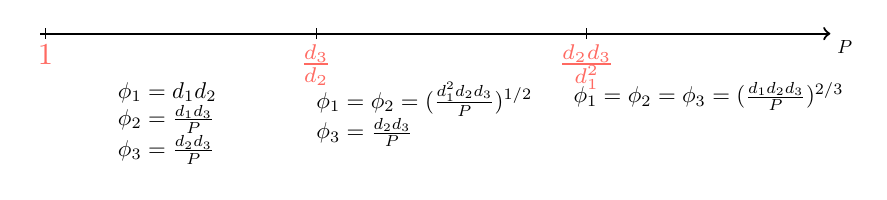
\begin{tikzpicture}[scale=0.6875, every node/.style={transform shape}]
		%%\draw (-2,0) -- node[below] {a} ++(2,0) -- node[above] {b} ++(2,0);
		%%\draw (-0.1,0) -- ++(5,0) -- ++(5,0);
		\draw [->, thick] (-0.1,0) -- (14.5,0) node [below right] {$P$};
		\draw (0, 0.1) -- node [below, pastelred, scale=1.6]{$1$}(0,-0.1);
		\draw (5, 0.1) -- node [below, pastelred, scale=1.6]{$\frac{d_3}{d_2}$}(5,-0.1);
		\draw (10, 0.1) -- node [below, pastelred, scale=1.6] {$\frac{d_2d_3}{d_1^2}$}(10,-0.1);
		
		\node[align=left,below,scale=1.2] at (2.25, -0.75) {$\phi_1 = d_1d_2$\\ $\phi_2=\frac{d_1d_3}{P}$\\ $\phi_3 = \frac{d_2d_3}{P}$};
		\node[align=left,below,scale=1.2] at (7, -0.75) {$\phi_1 =\phi_2= (\frac{d_1^2d_2d_3}{P})^{1/2}$\\ $\phi_3 = \frac{d_2d_3}{P}$};
		\node[align=center,below,scale=1.2] at (12.25, -0.75) {$\phi_1 = \phi_2 = \phi_3 = (\frac{d_1d_2d_3}{P})^{2/3}$};	
		\end{tikzpicture}
	\end{center} 
\end{block}
\begin{block}{\small Communication Lower Bounds (Amount of Data Transfers)}
	\begin{center}
	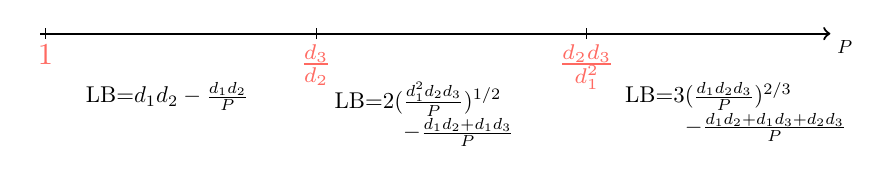
\begin{tikzpicture}[scale=0.6875, every node/.style={transform shape}]
	%%\draw (-2,0) -- node[below] {a} ++(2,0) -- node[above] {b} ++(2,0);
	%%\draw (-0.1,0) -- ++(5,0) -- ++(5,0);
	\draw [->, thick] (-0.1,0) -- (14.5,0) node [below right] {$P$};
	\draw (0, 0.1) -- node [below, pastelred, scale=1.6]{$1$}(0,-0.1);
	\draw (5, 0.1) -- node [below, pastelred, scale=1.6]{$\frac{d_3}{d_2}$}(5,-0.1);
	\draw (10, 0.1) -- node [below, pastelred, scale=1.6] {$\frac{d_2d_3}{d_1^2}$}(10,-0.1);
	
	\node[align=left,below,scale=1.2] at (2.25, -0.75) {LB=$d_1d_2 -\frac{d_1d_2}{P}$};
	\node[align=left,below,scale=1.2] at (7, -0.75) {LB=$2(\frac{d_1^2d_2d_3}{P})^{1/2}$\\
		$\qquad\quad-\frac{d_1d_2+d_1d_3}{P}$};
	\node[align=center,below,scale=1.2] at (12.25, -0.75) {LB=$3(\frac{d_1d_2d_3}{P})^{2/3}$\\ $\qquad\qquad\quad -\frac{d_1d_2+d_1d_3+d_2d_3}{P}$};	
	\end{tikzpicture}
\end{center}
\end{block}
\end{frame}


\begin{frame}{Design of Communication Optimal Algorithms}
\vspace*{-0.25cm}\begin{block}{\small Data Distribution ($P$ is organized into a $p_1 \times p_2 \times p_3$ grid)}
\begin{minipage}{0.75\linewidth}{\small	
	\begin{itemize}
		\item $p_1,p_2$, and $p_3$ evenly distribute $n_1, n_2$, and $n_3$
		\item Each processor has $\frac{1}{P}$th amount of input and output variables
		\item $A_{31} = A(2\frac{n_1}{p_1}+1:3\frac{n_1}{p_1}, 1:\frac{n_2}{p_2})$ is evenly distributed among $(3,1, *)$ processors
		\item $B_{12} =  B(1:\frac{n_2}{p_2}, \frac{n_3}{p_3}+1:2\frac{n_3}{p_3})$ is evenly distributed among $(*,1,2)$ processors  
	\end{itemize}
}\end{minipage}
\begin{minipage}{0.2\linewidth}
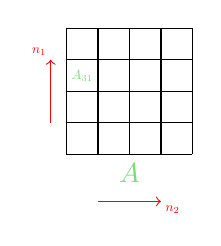
\begin{tikzpicture}[scale=0.4, every node/.style={transform shape}]
\def\xref{0.6}
\def\yref{0.5}

\foreach \y in {0, 1, 2, 3, 4}
\draw (-2, \y) -- (2, \y);

\foreach \x in {-2, -1, 0, 1, 2}
\draw (\x, 0) -- (\x, 4);

\node [below, pastelgreen, scale=2.5] at (0,0) {$A$};


\node [ pastelgreen, scale=1.2] at (-1.5,2.5) {$A_{31}$};

\draw [->, red] (-1,-1.5) -- (1,-1.5) node [below right, scale=1.2] {$n_2$};
\draw [->, red] (-2.5,1) -- (-2.5,3) node [ above left, scale=1.2] {$n_1$};
\end{tikzpicture}
\end{minipage}
\end{block}

	\vspace*{-0.3cm}\begin{algorithm}[H]{\footnotesize
		\caption{$C=AB$ Matrix Multiplication Algorithm}
		\begin{algorithmic}[1]
			\STATE $(p_1^\prime, p_2^\prime, p_3^\prime)$ is my processor id
			\STATE //All-gather input matrices $A$ and $B$
			\STATE $A_{p_1^\prime p_2^\prime}$ = All-Gather($A$, $(p_1^\prime, p_2^\prime, *)$)
			\STATE $B_{p_2^\prime p_3^\prime}$ = All-Gather($B$, $(*, p_2^\prime, p_3^\prime)$)
%%			\STATE //Perform local Matrix Multiplication in a temporary variable $T$
			\STATE $T$ = Local-Matrix-Multiplication($A_{p_1^\prime p_2^\prime}, B_{p_2^\prime p_3^\prime} $) // Local matrix multiplication in a temporary
%%			\STATE //Reduce-scatter the output matrix in $C_{p_1^\prime p_3^\prime}$
			\STATE Reduce-Scatter($C_{p_1^\prime p_3^\prime}$, T,  $(p_1^\prime,*,p_3^\prime)$) // Reduce-scatter the output
		\end{algorithmic}
}\end{algorithm}
\end{frame}
\begin{frame}{Cost Analysis and Open Questions}
\begin{block}{Cost Analysis}
	\begin{itemize}
		\item Total amount of multiplications per processor = $\frac{n_1n_2n_3}{p_1p_2p_3} = \frac{n_1n_2n_3}{P}$
%%		\item Amount of data transfers to perform All-Gather/Reduce-Scatter operation on $Q$ processors = $(1-\frac{1}{Q})w$, $w$ is amount of total data after All-Gather or before Reduce-Scatter operation
		\item Total data transfers = $\frac{n_1n_2}{p_1p_2} + \frac{n_2n_3}{p_2p_3} + \frac{n_1n_3}{p_1p_3} - \frac{n_1n_2+n_2n_3+n_1n_3}{P}$   
	\end{itemize}
\end{block}
\vfill
\begin{block}{Open Questions}
	\begin{itemize}
		\item How to select $p_1, p_2, p_3$?
		\item Are communication lower bounds are achievable for all matrix dimensions?
	\end{itemize}
\end{block}

\end{frame}

\section{For Multi-TTM Computation}

\begin{frame}{Outline}
\tableofcontents
\end{frame}
\setcounter{algorithm}{0}
\begin{frame}{Multi-TTM Computation}
\begin{itemize}
	\item $\T{X} \in \mathbb{R}^{n_1\times \cdots \times n_d}$: input tensor, $\T{Y}\in \mathbb{R}^{r_1\times\cdots \times r_d}$: output tensor
	\item $\Mn{A}{k}\in \mathbb{R}^{n_k\times r_k}$: factor matrix of the $k$th mode
\end{itemize}
\begin{block}{\small 2-dimensional Multi-TTM ($\Y = \X \times_1 {\Mn{A}{1}}^\Tra \times_2 {\Mn{A}{2}}^\Tra$)}
	TTM-in-Sequence approach (used in Tucker-MPI): $\M{Y} = \MnTra{A}{1}{}\M{X}\Mn{A}{2}$\\
	All-at-Once approach (our contribution):	
	 \vspace*{-0.25cm}\begin{align*}
	 &\text{for $n_1^\prime = 1{:}n_1$, for $n_2^\prime = 1{:}n_2$}\\
	 &\quad \text{for $r_1^\prime = 1{:}r_1$, for $r_2^\prime = 1{:}r_2$}\\
	 &\quad \quad \Y(r_1^\prime,r_2^\prime) = \Y(r_1^\prime,r_2^\prime) + \Big( \X(n_1^\prime,n_2^\prime) *  \Mn{A}{1}(n_{1}^\prime,r_1^\prime) * \Mn{A}{2}(n_2^\prime,r_2^\prime) \Big)
	 \end{align*}
\end{block}

%%\begin{itemize}
%%	\item TTM-in-sequence
%%	\item All-at-once definition
%%\end{itemize}
\end{frame}

\begin{frame}{3-dimensional Multi-TTM ($\Y = \X \times_1 {\Mn{A}{1}}^\Tra \times_2 {\Mn{A}{2}}^\Tra \times_3 {\Mn{A}{3}}^\Tra$)}
\begin{block}{\small All-at-Once 3-dimensional Multi-TTM Computation}
	\begin{minipage}{0.7\linewidth}{\small
	\vspace*{-0.25cm}\begin{align*}
	&\text{for $n_1^\prime = 1{:}n_1$, for $n_2^\prime = 1{:}n_2$, for $n_3^\prime = 1{:}n_3$}\\
	&\quad \text{for $r_1^\prime = 1{:}r_1$, for $r_2^\prime = 1{:}r_2$, for $r_3^\prime = 1{:}r_3$}\\
	&\quad \quad \Y(r_1^\prime,r_2^\prime,r_3^\prime) = \Y(r_1^\prime,r_2^\prime,r_3^\prime)\\
	&\qquad\qquad + \Big( \X(n_1^\prime,n_2^\prime,n_3^\prime) *  \Mn{A}{1}(n_{1}^\prime,r_1^\prime) * \Mn{A}{2}(n_2^\prime,r_2^\prime) * \Mn{A}{3}(n_3^\prime,r_3^\prime)\Big)
	\end{align*}
	}\end{minipage}
	\begin{minipage}{0.25\linewidth}{\small
$\M{\Delta} = \begin{bmatrix}\M{I}_{3\times 3} & \V{1}_3 & \V{0}_3\\ \M{I}_{3\times 3} & \V{0}_3 & \V{1}_3 \end{bmatrix}$
}\end{minipage}
\end{block}
\begin{itemize}
	\item Total number of $4-array$ operations = $n_1r_1n_2r_2n_3r_3$
	\item $\M{\Delta}$ is not full rank
	\begin{itemize}
		\item Consider each vector $\V{x}$ such that $\M{\Delta}\cdot\V{x}=\V{1}$, $\V{x}$ is of the form [$a$ $a$ $a$ $1$-$a$ $1$-$a$]$^\Tra$ and $0\le a\le 1$
	\end{itemize}
	\item $\phi_{\X}$, $\phi_{\Y}$: tensor projections \& $\phi_1, \phi_2, \phi_3$: matrix projections
	\item From HBL, $\phi_{\X}^{1-a}\phi_{\Y}^{1-a} \phi_1^a \phi_2^a \phi_3^a \ge \text{Amount of computations}$
\end{itemize}
\end{frame}

\begin{frame}{Solving Optimization Problem to Compute Lower Bounds}
\begin{itemize}
	\item Select a processor which performs $\frac{n_1r_1n_2r_2n_3r_3}{P}$ amount of $4-array$ operations
	\item After applying lower and upper bounds for each projection, we need to solve the following optimization problem
\end{itemize}
\vspace*{-0.35cm}\begin{align*}
Minimize \ \phi_{\X} + \phi_{\Y} +& \phi_1 + \phi_2 + \phi_3 \  \text{ s.t.}\\
\phi_{\X}^{1-a}\phi_{\Y}^{1-a} \phi_1^a \phi_2^a \phi_3^a & \ge \frac{n_1r_1n_2r_2n_3r_3}{P}\\
\frac{n_1n_2n_3}{P} \le & \phi_{\X} \le n_1n_2n_3\\
\frac{r_1r_2r_3}{P} \le & \phi_{\Y} \le r_1r_2r_3\\
\frac{n_1r_1}{P} \le &\phi_1 \le n_1r_1\\
\frac{n_2r_2}{P} \le &\phi_2 \le n_2r_2\\
\frac{n_3r_3}{P} \le &\phi_3 \le n_3r_3
\end{align*}
\end{frame}
\begin{frame}{Divide the problem into two parts}
\vspace*{-0.25cm}
\begin{minipage}{0.45\linewidth}
	\begin{block}{Matrix part}{\small
		\vspace*{-0.45cm}\begin{align*}
		Minimize \ & \phi_1 + \phi_2 + \phi_3 \  \text{ s.t.}\\
		\phi_1 \phi_2 \phi_3 & \ge \frac{n_1r_1n_2r_2n_3r_3}{P}\\
		\frac{n_1r_1}{P} \le &\phi_1 \le n_1r_1\\
		\frac{n_2r_2}{P} \le &\phi_2 \le n_2r_2\\
		\frac{n_3r_3}{P} \le &\phi_3 \le n_3r_3
		\end{align*}
	}\end{block}
\end{minipage}$\quad$
\begin{minipage}{0.45\linewidth}
	\begin{block}{Tensor part}{\small
		\begin{align*}
		Minimize \ & \phi_{\X} + \phi_{\Y}\  \text{ s.t.}\\
		\phi_{\X}\phi_{\Y} & \ge \frac{n_1r_1n_2r_2n_3r_3}{P}\\
		\frac{n_1n_2n_3}{P} \le & \phi_{\X} \le n_1n_2n_3\\
		\frac{r_1r_2r_3}{P} \le & \phi_{\Y} \le r_1r_2r_3
		\end{align*}
	}\end{block}
\end{minipage}


\end{frame}
\begin{frame}{Amount of Accesses and Lower bounds}
\begin{itemize}{\small
		\item We assume $n_1r_1\le n_2r_2\le n_3r_3$ and $r_1r_2r_3\le n_1n_2n_3$
		\item Estimate solutions for both parts using Lagrange multipliers ( optimality can be proven using KKT conditions) 
}\end{itemize}
\vspace*{-0.25cm}\begin{block}{Amount of accesses = $\phi_{\X} + \phi_{\Y} + \phi_1 + \phi_2 + \phi_3$}
	\begin{center}
		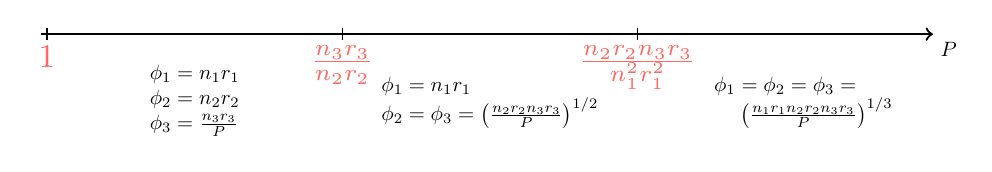
\begin{tikzpicture}[scale=0.75, every node/.style={transform shape}]
		%%\draw (-2,0) -- node[below] {a} ++(2,0) -- node[above] {b} ++(2,0);
		%%\draw (-0.1,0) -- ++(5,0) -- ++(5,0);
		\draw [->, thick] (-0.1,0) -- (15,0) node [below right] {$P$};
		\draw (0, 0.1) -- node [below, pastelred, scale=1.6]{$1$}(0,-0.1);
		\draw (5, 0.1) -- node [below, pastelred, scale=1.6]{$\frac{n_3r_3}{n_2r_2}$}(5,-0.1);
		\draw (10, 0.1) -- node [below, pastelred, scale=1.6] {$\frac{n_2r_2n_3r_3}{n_1^2r_1^2}$}(10,-0.1);
		
		\node[align=left,below] at (2.5, -0.4) {$\phi_1=n_1r_1$\\ $\phi_2=n_2r_2$\\ $\phi_3=\frac{n_3r_3}{P}$};
		\node[align=left,below] at (7.5, -0.6) {$\phi_1=n_1r_1$\\$\phi_2=\phi_3= \big(\frac{n_2r_2n_3r_3}{P}\big)^{1/2}$};
		\node[align=center,below] at (12.5, -0.6) {$\phi_1=\phi_2=\phi_3=$\\ $\qquad\quad \big(\frac{n_1r_1n_2r_2n_3r_3}{P}\big)^{1/3}$};	
		\end{tikzpicture}
	\end{center}
	
	\begin{center}
		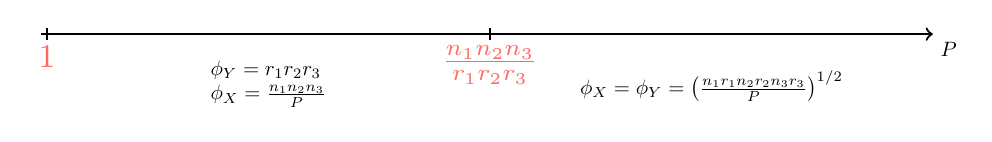
\begin{tikzpicture}[scale=0.75, every node/.style={transform shape}]
		\draw [->, thick] (-0.1,0) -- (15,0) node [below right] {$P$};
		\draw (0, 0.1) -- node [below, pastelred, scale=1.6]{$1$}(0,-0.1);
		\draw (7.5, 0.1) -- node [below, pastelred, scale=1.6]{$\frac{n_1n_2n_3}{r_1r_2r_3}$}(7.5,-0.1);
		
		\node[align=left,below] at (3.75, -0.325) {$\phi_{\Y}= r_1r_2r_3$\\ $\phi_{\X} = \frac{n_1n_2n_3}{P}$};
		\node[align=left,below] at (11.25, -0.5) {$\phi_{\X}=\phi_{\Y}= \big(\frac{n_1r_1n_2r_2n_3r_3}{P}\big)^{1/2}$};
		\end{tikzpicture}
	\end{center}
\end{block}
Communication lower bound = $\phi_{\X} + \phi_{\Y} + \phi_1 + \phi_2 + \phi_3 -\frac{n_1n_2n_3+r_1r_2r_3+n_1r_1+n_2r_2+n_3r_3}{P}$
\end{frame}
\begin{frame}{Design of Communication Optimal Algorithms}
	\begin{block}{\small Data Distribution ($P$ is organized into a $p_1 \times p_2 \times p_3\times q_1 \times q_2 \times q_3$ grid)}{\small
%%		\begin{minipage}{0.75\linewidth}{\small	
				\begin{itemize}
					\item $p_1,p_2, p_3, q_1, q_2$, and $q_3$ evenly distribute $n_1, n_2, n_3, r_1, r_2$, and  $r_3$
					\item Each processor has $\frac{1}{P}$th amount of input and output variables
					\item Subtensor $\T{X}_{231} = \T{X}(\frac{n_1}{p_1}+1:2\frac{n_1}{p_1}, 2\frac{n_2}{p_2}+1:3\frac{n_2}{p_2}, 1:\frac{n_3}{p_3})$ is distributed evenly among processors $(2,3,1,*,*,*)$ 
					\item Submatrix $\Mn{A}{2}_{31} = \Mn{A}{2}(2\frac{n_2}{p_2}+1:3\frac{n_2}{p_2}, 1:\frac{r_2}{q_2})$ is distributed evenly among processors $(*,3,*,*,1,*)$
				\end{itemize}
%%		}\end{minipage}
		\begin{center}
		\vspace*{-0.25cm}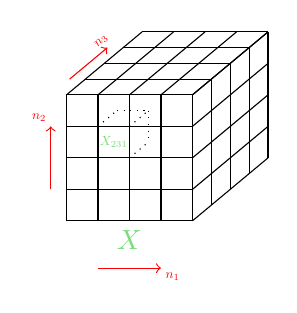
\begin{tikzpicture}[scale=0.4, every node/.style={transform shape}]
		\def\xref{0.6}
		\def\yref{0.5}
		
		\foreach \y in {0, 1, 2, 3, 4}
		\draw (-2, \y) -- (2, \y);
		
		\foreach \x in {-2, -1, 0, 1, 2}
		\draw (\x, 0) -- (\x, 4);
		
		\foreach \y in {0, 1, 2, 3, 4}
		\draw (2, \y)--(2+4*\xref, 4*\yref+\y);
		
		
		\foreach \y in {0, 1, 2, 3, 4}
		\draw (2+\y * \xref, \y * \yref) -- (2+\y * \xref, 4+\y * \yref);
		
		\foreach \x in {-2, -1, 0, 1, 2}
		\draw (\x, 4) -- (\x + 4*\xref, 4+4*\yref);
		
		\foreach \y in {0, 1, 2, 3, 4}
		\draw (-2+\y * \xref, 4+\y * \yref) -- (2+\y * \xref, 4+\y * \yref);
		
		\node [below, pastelgreen, scale=2.5] at (0,0) {$\T{X}$};
		
		\draw [dotted] (-1, 3) -- (-1+\xref,3+\yref);
		\draw [dotted] (0, 3) -- (0+\xref,3+\yref);
		\draw [dotted] (0, 2) -- (0+\xref,2+\yref);
		\draw [dotted] (-1+\xref,3+\yref) -- (0+\xref,3+\yref);
		\draw [dotted] (0+\xref,3+\yref) -- (0+\xref,2+\yref);
		
		\node [ pastelgreen, scale=1.2] at (-0.5,2.5) {$\T{X}_{231}$};
		
		\draw [->, red] (-1,-1.5) -- (1,-1.5) node [below right, scale=1.2] {$n_1$};
		\draw [->, red] (-2.5,1) -- (-2.5,3) node [ above left, scale=1.2] {$n_2$};
		\draw [->, red] (-2.5+\xref, 4+\yref) -- (-2.5 + 3*\xref, 4+3*\yref) node [above,rotate=45, scale=1.2] {$n_3$};
		\end{tikzpicture}$\qquad$
		\vspace*{-0.25cm}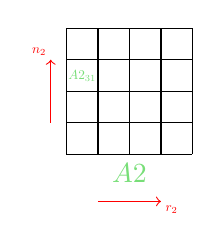
\begin{tikzpicture}[scale=0.4, every node/.style={transform shape}]
		\def\xref{0.6}
		\def\yref{0.5}
		
		\foreach \y in {0, 1, 2, 3, 4}
		\draw (-2, \y) -- (2, \y);
		
		\foreach \x in {-2, -1, 0, 1, 2}
		\draw (\x, 0) -- (\x, 4);
		
		\node [below, pastelgreen, scale=2.5] at (0,0) {$\Mn{A}{2}$};
		
		
		\node [ pastelgreen, scale=1.2] at (-1.5,2.5) {$\Mn{A}{2}_{31}$};
		
		\draw [->, red] (-1,-1.5) -- (1,-1.5) node [below right, scale=1.2] {$r_2$};
		\draw [->, red] (-2.5,1) -- (-2.5,3) node [ above left, scale=1.2] {$n_2$};
		\end{tikzpicture}
		\end{center}
	\vspace*{-0.15cm}
	}\end{block}
\end{frame}
\begin{frame}{6-dimensional Algorithm to compute Multi-TTM}
\vspace*{-0.35cm}\begin{algorithm}[H]
	\caption{3-dimensional Parallel Atomic Multi-TTM}
	\begin{algorithmic}[1]
		\REQUIRE $\T{X}$, $\Mn{A}{1}$, $\Mn{A}{2}$, $\Mn{A}{3}$, $p_1 \times p_2 \times p_3 \times q_1 \times q_2 \times q_3$ logical processor grid
		\ENSURE $\T{Y}$ such that $\Y = \X \times_1 {\Mn{A}{1}}^\Tra \times_2 {\Mn{A}{2}}^\Tra \times_3 {\Mn{A}{3}}^\Tra$
		\STATE $(p_1^\prime, p_2^\prime, p_3^\prime, q_1^\prime, q_2^\prime, q_3^\prime)$ is my processor id
		\STATE //All-gather input tensor and matrices
		\STATE $\T{X}_{p_1^\prime p_2^\prime p_3^\prime}$ = All-Gather($\T{X}$, $(p_1^\prime, p_2^\prime, p_3^\prime, *, *, *)$)\label{alg:3dmultittm:line:allGatherInputTensor}
		\STATE $\Mn{A}{1}_{p_1^\prime q_1^\prime}$ = All-Gather($\Mn{A}{1}$, $(p_1^\prime, *, *, q_1^\prime, *, *)$)\label{alg:3dmultittm:line:allGatherMatrix1}
		\STATE $\Mn{A}{2}_{p_2^\prime q_2^\prime}$ = All-Gather($\Mn{A}{2}$, $(*, p_2^\prime, *, *, q_2^\prime, *)$)\label{alg:3dmultittm:line:allGatherMatrix2}
		\STATE $\Mn{A}{3}_{p_3^\prime q_3^\prime}$ = All-Gather($\Mn{A}{3}$, $(*, *, p_3^\prime, *, *, q_3^\prime)$)
		\STATE //Perform local Multi-TTM computation in a temporary tensor $\T{T}$
		\STATE $\T{T}$ = Local-Multi-TTM($\T{X}_{p_1^\prime p_2^\prime p_3^\prime}$, $\Mn{A}{1}_{p_1^\prime q_1^\prime}$, $\Mn{A}{2}_{p_2^\prime q_2^\prime}$, $\Mn{A}{3}_{p_3^\prime q_3^\prime}$)
		\STATE //Reduce-scatter the output tensor in $\T{Y}_{q_1^\prime q_2^\prime q_3^\prime}$
		\STATE Reduce-Scatter($\T{Y}_{q_1^\prime q_2^\prime q_3^\prime}$, $\T{T}$, $(*, *, *, q_1^\prime, q_2^\prime, q_3^\prime)$)
	\end{algorithmic}
\end{algorithm}
\end{frame}
\begin{frame}{Cost Analysis of our Algorithm}
	\begin{itemize}
		\item Total amount of $4$-array operations per processor = $\frac{n_1r_1n_2r_2n_3r_3}{p_1q_1p_2q_2p_3q_3} = \frac{n_1r_1n_2r_2n_3r_3}{P}$
		\vfill
		\item Data transfers happen only in All-Gather and Reduce-Scatter collective operations
		\begin{itemize}
			\item Cost on $Q$ processors is $(1-\frac{1}{Q})w$, $w$ is the amount of total data after All-Gather or before Reduce-Scatter operation 
		\end{itemize}
		\vfill
		%%		\item Amount of data transfers to perform All-Gather/Reduce-Scatter operation on $Q$ processors = $(1-\frac{1}{Q})w$, $w$ is amount of total data after All-Gather or before Reduce-Scatter operation
		\item Total data transfers = $\frac{n_1n_2n_3}{p_1p_2p_3} + \frac{r_1r_2r_3}{q_1q_2q_3} + \frac{n_1r_1}{p_1q_1} +\frac{n_2r_2}{p_2q_2} + \frac{n_3r_3}{p_3q_3} - \frac{n_1n_2n_3+r_1r_2r_3+n_1r_1+n_2r_2+n_3r_3}{P}$
		\vfill
		\item $p_1, p_2, p_3, q_1, q_2$, and $q_3$ can be obtained based on lower bounds (Not today)  
	\end{itemize}
\end{frame}
\subsection{Simulated Experiments}
\begin{frame}{Outline}
\tableofcontents[currentsubsection]
\end{frame}

\begin{frame}{Communication Lower Bound ($\lowerbound$) distributions}
\begin{minipage}{0.475\linewidth}
	\begin{block}{$n_1=n_2=n_3=2^{12},r_1=r_2=r_3=2^{4}$}
		\begin{center}
			\includegraphics[scale=0.56]{./LB-logscale-12-12-12-4-4-4.eps}
		\end{center}
	\end{block}
\end{minipage}$\quad$
\begin{minipage}{0.475\linewidth}
	\begin{block}{$n_1=n_2=n_3=2^{20},r_1=r_2=r_3=2^{8}$}
		\begin{center}
			\includegraphics[scale=0.56]{./LB-logscale-20-20-20-8-8-8.eps}
		\end{center}
	\end{block}
\end{minipage}
%%\begin{figure*}[htb]
%%	\begin{center}
%%		\subfloat[$n_1=2^{12}, n_2=2^{13}, n_3=2^{19},r_1=2^{8},r_2=2^{13}, r_3=2^{11}$.\label{fig:lb:allcases}]{\includegraphics[width=0.32\linewidth]{./LB-logscale-12-13-19-8-13-11.eps}}\hfill
%%		\subfloat[$n_1=n_2=n_3=2^{12},r_1=r_2=r_3=2^{4}$.\label{fig:lb:matrixdominated}]{\includegraphics[width=0.32\linewidth]{./LB-logscale-12-12-12-4-4-4.eps}}\hfill	
%%		\subfloat[$n_1=n_2=n_3=2^{20},r_1=r_2=r_3=2^{8}$.\label{fig:lb:genpattern}]{\includegraphics[width=0.32\linewidth]{./LB-logscale-20-20-20-8-8-8.eps}}
%%		\vspace*{-0.05cm}\caption{Matrix and tensor communication costs in Multi-TTM communication lower bounds ($\lowerbound$) for different configurations.\label{fig:lb}\vspace*{-0.15cm}}
%%	\end{center}
%%\end{figure*}
\begin{itemize}
	\item Matrix communication costs dominate when $P$ is much less than $\frac{n_1n_2n_3}{r_1r_2r_3}$
\end{itemize}
\
\end{frame}
\begin{frame}{Performance Comparison of Our Algorithm}
\begin{minipage}{0.475\linewidth}
\begin{block}{$n_1=n_2= n_3=2^{20},r_1=r_2=r_3=2^{8}$}
	\begin{center}
		\includegraphics[scale=0.45]{./A@O-vs-Seq-logscale-20-20-20-8-8-8.eps}
	\end{center}
\end{block}
\end{minipage}$\quad$
\begin{minipage}{0.475\linewidth}
	\begin{block}{$n_1=n_2= n_3=2^{12},r_1=r_2=r_3=2^{4}$}
		\begin{center}
			\includegraphics[scale=0.45]{./A@O-vs-Seq-logscale-12-12-12-4-4-4.eps}
		\end{center}
	\end{block}
\end{minipage}
%%\begin{itemize}{
{\small$\bullet$ $C_{LB}$: Communication lower bound, \bestconfigAAO: Our algorithm with the best partition, \lbbasedpartition: Our algorithm with the partition based on the lower bound, \bestconfigSeq: Multi-TTM computation used in Tucker-MPI with the best partition\\
$\bullet$ Our algorithm communicates much less than the approach in Tucker-MPI
}
%%	\item The gap between our algorithm and \bestconfigSeq is large at the second kink in \bestconfigSeq (more than $10\time$)
%%\end{itemize}
\end{frame}

\subsection{Conclusion}
\begin{frame}{Outline}
\tableofcontents[currentsubsection]
\end{frame}

	
 \begin{frame}{Conclusion and Future Work}
\begin{block}{Conclusion}
	\begin{itemize}
		\item Lower bounds for All-at-Once Multi-TTM
		\item Communication Optimal Algorithm for Multi-TTM
		\item Comparison of our algorithm with the TTM-in-Sequence Algorithm
		\item Our algorithm communicates much less data than TTM-in-Sequence for $P < \frac{n_1n_2n_3}{r_1r_2r_3}$ 
	\end{itemize}
\end{block}
\vfill
\begin{block}{Future Work}
	\begin{itemize}
		\item Detailed study of what scenarios are favorable for our algorithm
		\item Combine both All-at-Once and TTM-in-Sequence approaches to minimize communication lower bounds
		\item Extend our work for the full Tucker-decomposition algorithms
		
	\end{itemize}
\end{block}
\end{frame}



\end{document} 